% !TeX program = xelatex
% 自中午第三章圖片修訂起，現行 22 張圖之完整插入片段。
% 由 build_overleaf_handoff.py 從唯一分節正文產生；不在本檔另改圖說。
% 分節正文已含圖：整節替換時，不再重複貼入本檔。
% 本檔供逐段複製，不是可整份 input 的額外章節。
% 圖號由 LaTeX 自動產生，勿手寫 3-1、3-2 等數字。

% ==================================================
% 3.1.1 旋轉群與角度參數比較
% 位置：3.1.1 末尾、3.1.2 之前；說明為何採用旋轉群表示之後
% 正文來源：03_01_kinematics.tex
% 同名 PDF 請覆蓋上傳；同名 label 只保留一份。
% ==================================================
旋轉群與角度參數的表示差異如\cref{fig:ref_rotation_representation}所示。角度在選定的主值區間邊界會出現包絡跳變，對應的旋轉矩陣則維持連續。此圖說明本研究採用幾何位姿表示的背景；底盤的全向運動模型仍依本研究輪系建立。
\begin{figure}[htbp]
    \centering
    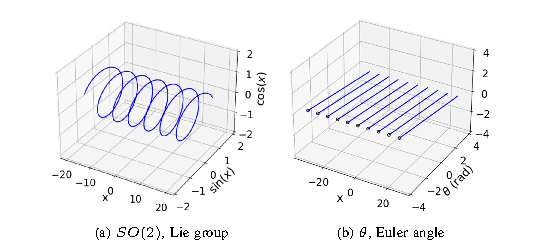
\includegraphics[width=0.95\textwidth]{figsrc/reference_figures/rotation_representation_tang2024.pdf}
    \caption{旋轉群與角度參數表示之比較：(a) $\mathrm{SO}(2)$ 旋轉群表示；(b) 歐拉角參數表示（引自文獻\cite{tang2024gmpc}之圖~1）。}
    \label{fig:ref_rotation_representation}
\end{figure}


% ==================================================
% 3.1.2 底盤參考與實際位姿
% 位置：3.1.2 幾何誤差及局部模型的公式與說明之後
% 正文來源：03_01_kinematics.tex
% 同名 PDF 請覆蓋上傳；同名 label 只保留一份。
% ==================================================
底盤位姿的相對幾何關係如\cref{fig:ch3_base_pose_error}所示。圖中 $t_E=R_r^{\top}(p_B-p_r)$ 為相對變換的平移分量；幾何誤差 $e_B$ 則由完整相對位姿的對數映射取得，兩者依各自定義使用。
\begin{figure}[htbp]
    \centering
    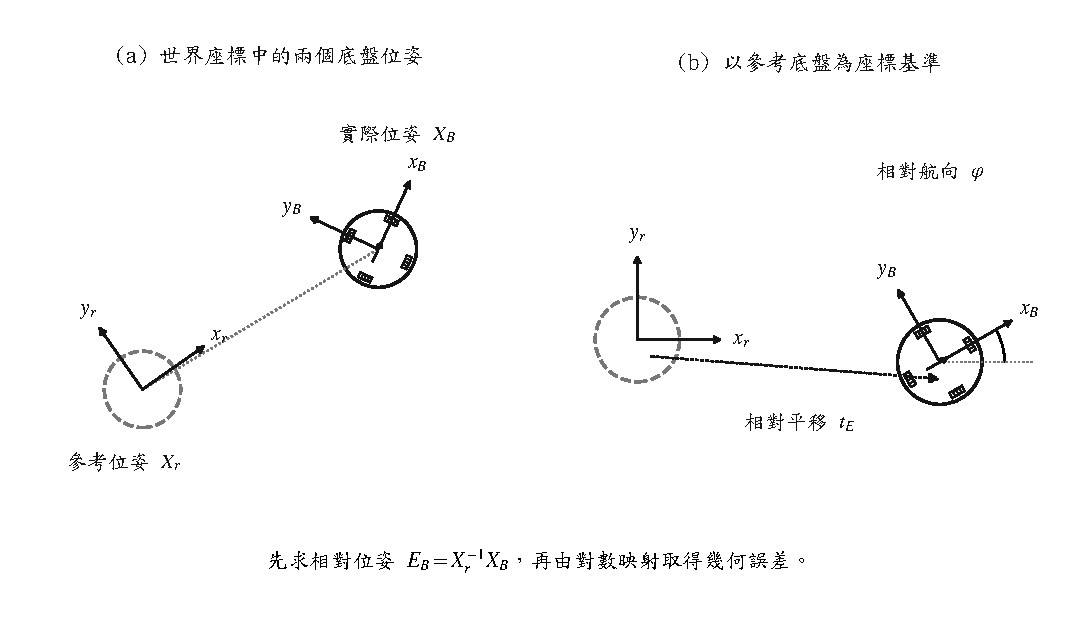
\includegraphics[width=0.98\textwidth]{figsrc/ch03/base_pose_error.pdf}
    \caption{底盤追蹤之相對幾何關係：(a) 世界座標中的參考與實際底盤位姿；(b) 以參考底盤為基準的相對平移與航向。}
    \label{fig:ch3_base_pose_error}
\end{figure}


% ==================================================
% 3.1.3 底盤側移與手臂補償
% 位置：3.1.3 全身正向運動學、雅可比矩陣說明之後
% 正文來源：03_01_kinematics.tex
% 同名 PDF 請覆蓋上傳；同名 label 只保留一份。
% ==================================================
底盤與手臂的運動學耦合如\cref{fig:ch3_wholebody_motion_coupling}所示。兩個構型對應相同的世界座標末端目標；底盤側移時，手臂配合調整關節構型，使末端保持在操作目標附近。
\begin{figure}[htbp]
    \centering
    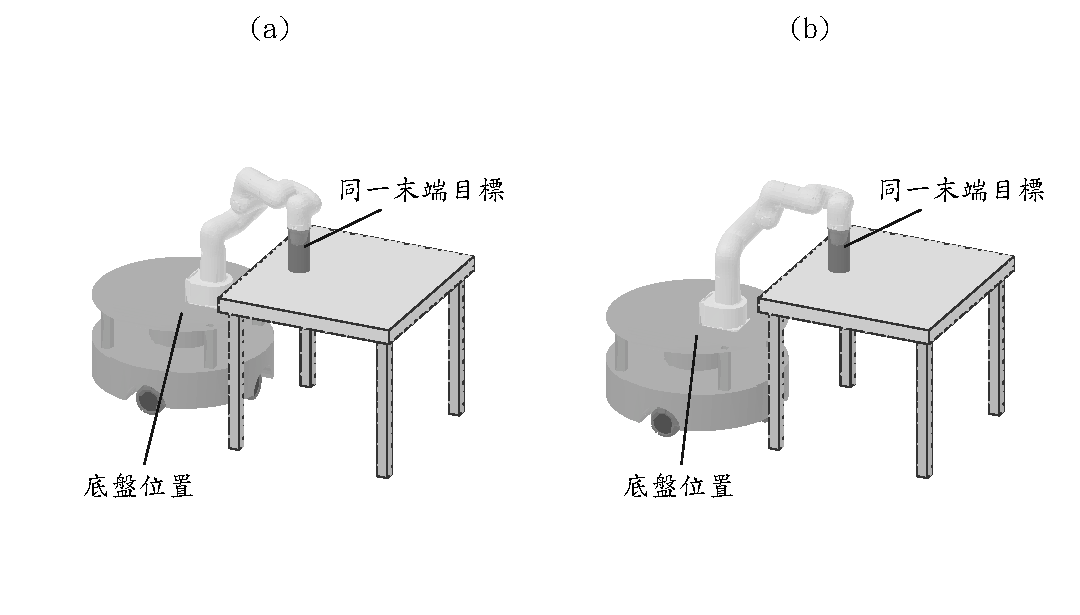
\includegraphics[width=0.98\textwidth]{figsrc/ch03/wholebody_motion_coupling.pdf}
    \caption{底盤側移時之全身運動學耦合：(a) 底盤移動前；(b) 底盤側移後，手臂調整構型以維持相同末端目標。}
    \label{fig:ch3_wholebody_motion_coupling}
\end{figure}


% ==================================================
% 3.2.2 設定點與實際關節追蹤
% 位置：3.2.2 增廣狀態及設定點／實際位置差異的說明之後
% 正文來源：03_02_augmented_prediction.tex
% 同名 PDF 請覆蓋上傳；同名 label 只保留一份。
% ==================================================
位置設定點與實際關節位置的追蹤關係如\cref{fig:ch3_arm_setpoint_tracking}所示。圖中以單軸一階追蹤模型呈現設定點固定後，實際關節仍逐步接近設定點的情形，說明預測時需分別保留實際關節位置 $q_a$ 與位置設定點 $s_a$。
\begin{figure}[htbp]
    \centering
    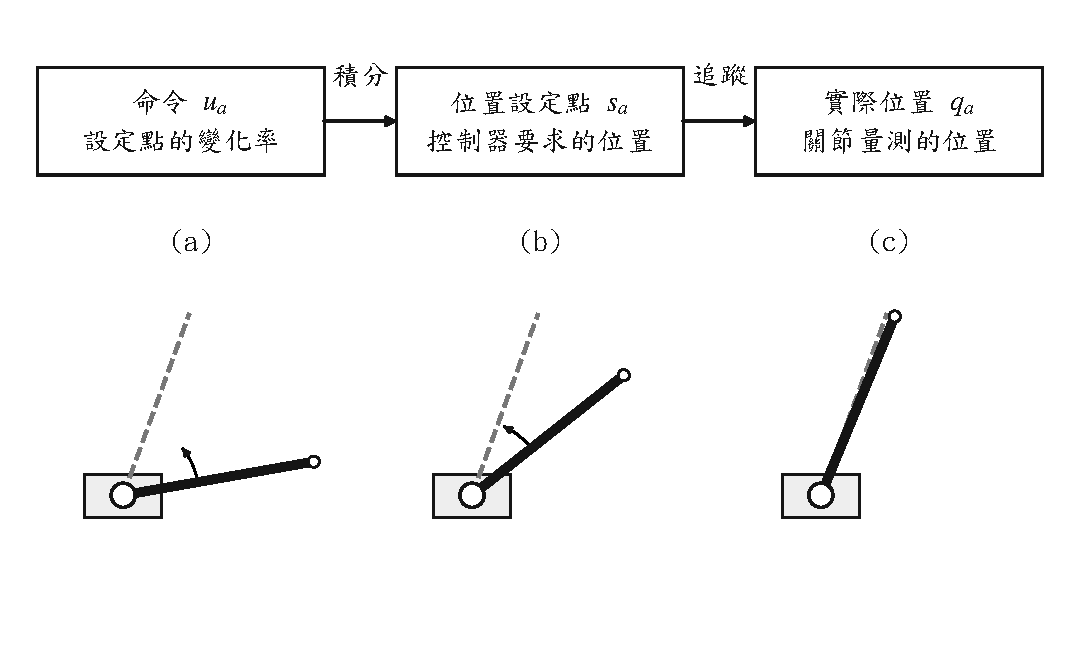
\includegraphics[width=0.98\textwidth]{figsrc/ch03/arm_setpoint_tracking.pdf}
    \caption{手臂設定點與實際關節位置之追蹤關係：(a) 設定點固定；(b) 關節持續追蹤；(c) 關節逐漸接近設定點。虛線與實線分別表示位置設定點與實際關節位置。}
    \label{fig:ch3_arm_setpoint_tracking}
\end{figure}


% ==================================================
% 3.3.2 十字全向輪速度可行域
% 位置：3.3.2 輪速限制、可行域推導及超限例子之後
% 正文來源：03_03_objective_constraints.tex
% 同名 PDF 請覆蓋上傳；同名 label 只保留一份。
% ==================================================
因此，固定旋轉速度下的平移可行域為軸向方框，其邊界隨 $|\omega|$ 增加而縮小；在 $v_y=0$ 的 $v_x$--$\omega$ 剖面則呈菱形，如\cref{fig:ch3_omni_velocity_feasible_set}所示。以 $r_w=0.05$ m、$L=0.245$ m 與 $\bar\omega_w=5.55$ rad/s 為例，獨立速度框內的 $v_x=0.24$ m/s、$\omega=0.8$ rad/s 需要的輪緣速度達 $0.436$ m/s，超過 $0.2775$ m/s 上限。圖中使用未內縮之幾何界限，實驗中的控制餘裕及輪加速度限制另行列示。
\begin{figure}[htbp]
    \centering
    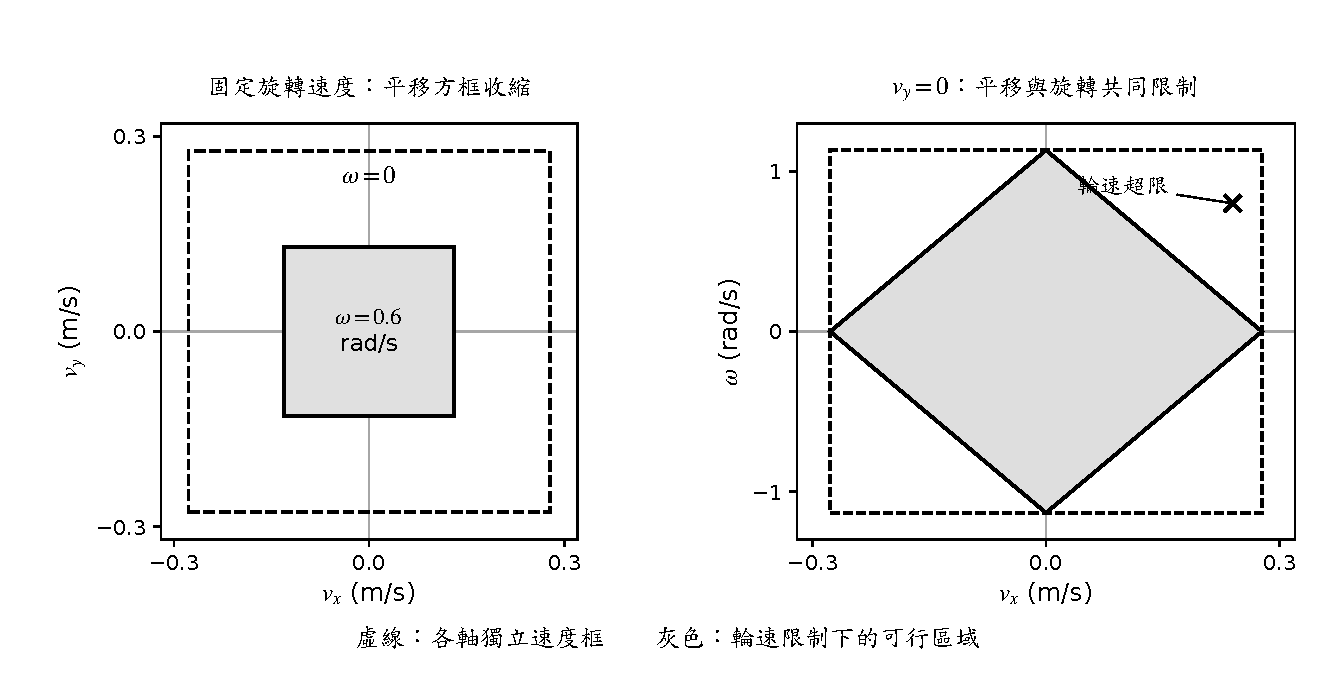
\includegraphics[width=0.98\textwidth]{figsrc/ch03/omni_wheel_velocity_feasible_set.pdf}
    \caption{四輪十字配置之速度可行域：(a) 固定旋轉速度下的 $v_x$--$v_y$ 平移可行域；(b) $v_y=0$ 時的 $v_x$--$\omega$ 剖面。虛線表示各軸獨立速度框，灰色表示輪速限制下的可行區域。}
    \label{fig:ch3_omni_velocity_feasible_set}
\end{figure}


% ==================================================
% 3.3.3 底盤與手臂共同求解
% 位置：3.3.3 QP 建構與數值求解說明之後
% 正文來源：03_03_objective_constraints.tex
% 同名 PDF 請覆蓋上傳；同名 label 只保留一份。
% ==================================================
共同求解的輸入與輸出關係如\cref{fig:ch3_joint_optimization}所示。導航參考與末端操作目標共同作用於同一控制序列，配合增廣模型及限制條件，同時決定底盤速度命令與手臂設定點變化率。
\begin{figure}[htbp]
    \centering
    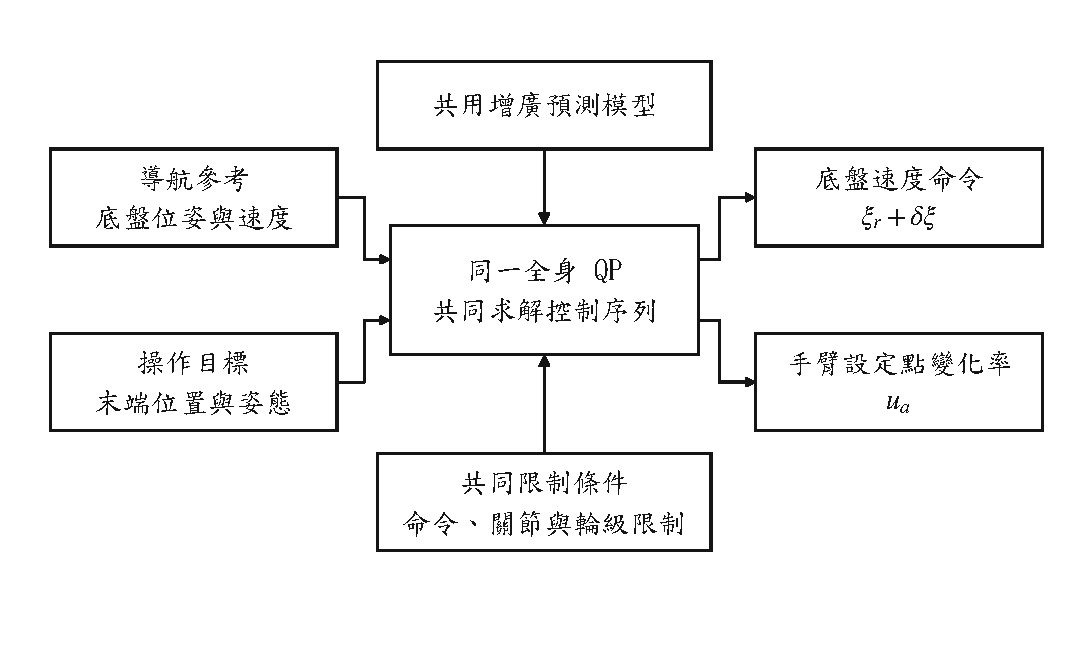
\includegraphics[width=0.98\textwidth]{figsrc/ch03/joint_optimization.pdf}
    \caption{底盤與手臂於同一全身控制問題中共同求解}
    \label{fig:ch3_joint_optimization}
\end{figure}


% ==================================================
% 3.4.1 卡爾曼預測與量測更新
% 位置：3.4.1 等速度模型與量測模型的公式之後；保留本文符號對照段
% 正文來源：03_04_dynamic_obstacle_avoidance.tex
% 同名 PDF 請覆蓋上傳；同名 label 只保留一份。
% ==================================================
卡爾曼濾波的預測與量測更新流程如\cref{fig:ref_kalman_predict_update}所示。圖中的 $A$ 與 $H$ 分別對應本節的 $F_o(\Delta\tau)$ 與 $H_o$；障礙物運動未設定外部控制輸入，因此圖中的 $Bu$ 項取零。追蹤器先將位置與速度向前預測，再以新群集中心量測修正估計。
\begin{figure}[htbp]
    \centering
    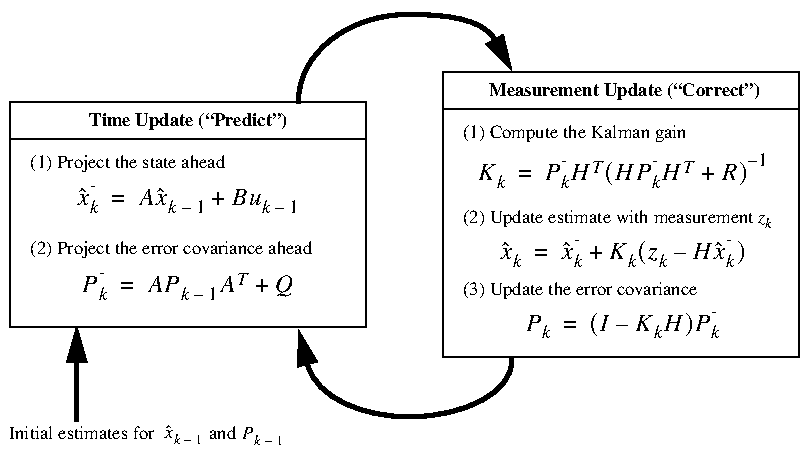
\includegraphics[width=0.98\textwidth]{figsrc/reference_figures/kalman_predict_update_welch2004.pdf}
    \caption{卡爾曼濾波之預測與量測更新流程（引自文獻\cite{welch2004kalman}之圖~1-2）}
    \label{fig:ref_kalman_predict_update}
\end{figure}


% ==================================================
% 3.4.2 原速度、減速與側移預測
% 位置：3.4.2 最小預測間距的公式及候選說明之後
% 正文來源：03_04_dynamic_obstacle_avoidance.tex
% 同名 PDF 請覆蓋上傳；同名 label 只保留一份。
% ==================================================
不同候選運動與行人的預測位置如\cref{fig:ch3_dynamic_obstacle_prediction}所示。(a) 為目前觀測，(b) 至 (d) 分別比較原速度、減速與側移在相同未來時刻的位置。減速改變抵達交會區的時間，側移則改變通行位置；實際候選評估依式\eqref{eq:ch3_candidate_clearance_margin}共同考量各障礙與全部選定取樣時刻。
\begin{figure}[htbp]
    \centering
    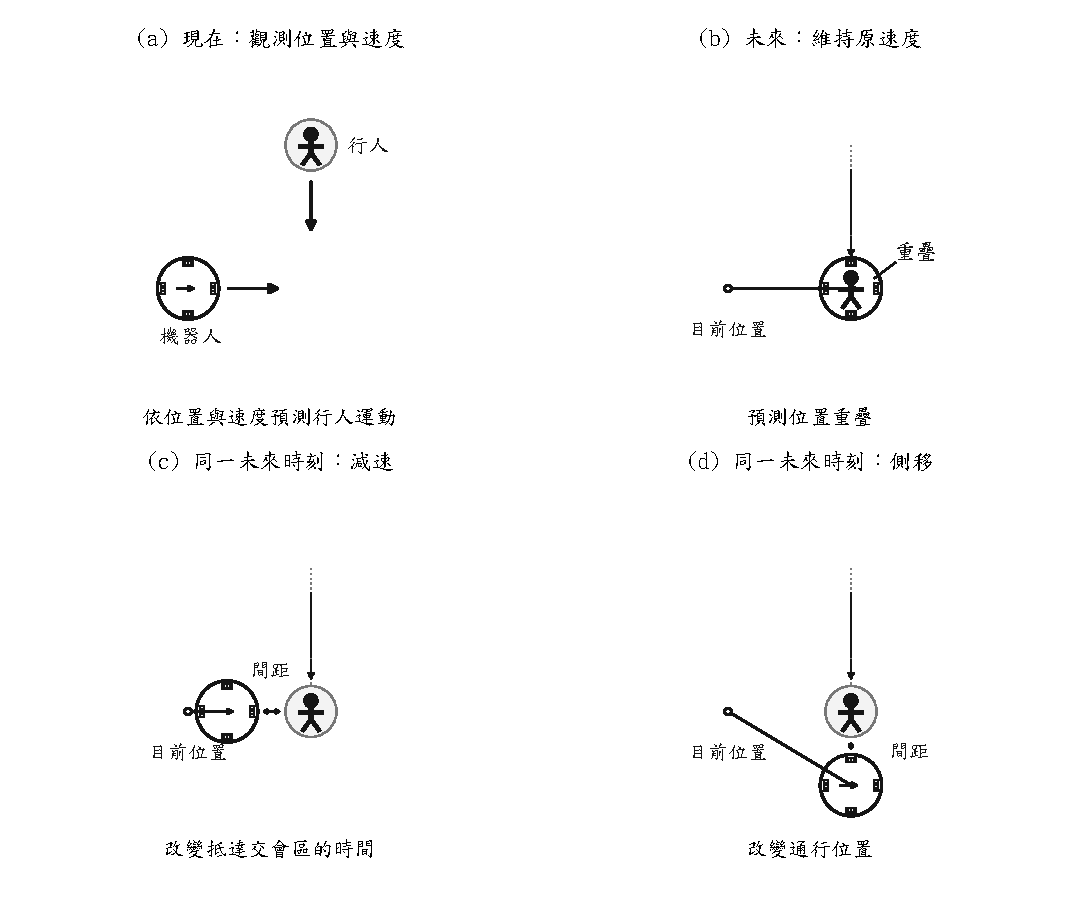
\includegraphics[width=0.98\textwidth]{figsrc/ch03/dynamic_obstacle_prediction.pdf}
    \caption{同一未來時刻下的候選運動比較：(a) 目前觀測；(b) 維持原速度；(c) 降低速度；(d) 側向避讓。}
    \label{fig:ch3_dynamic_obstacle_prediction}
\end{figure}


% ==================================================
% 3.4.5 導航與命令處理分層
% 位置：3.4.5 原始雷射防護與輪級命令處理說明之後
% 正文來源：03_04_dynamic_obstacle_avoidance.tex
% 同名 PDF 請覆蓋上傳；同名 label 只保留一份。
% ==================================================
各層的作用位置如\cref{fig:ch3_navigation_command_layers}所示。參考調整改變導航目標序列，CBF 作用於全身最佳化問題，雷射防護與輪級限制則依序處理待執行底盤命令；最終放行值回報後，供後續命令限制與運動預測使用。
\begin{figure}[htbp]
    \centering
    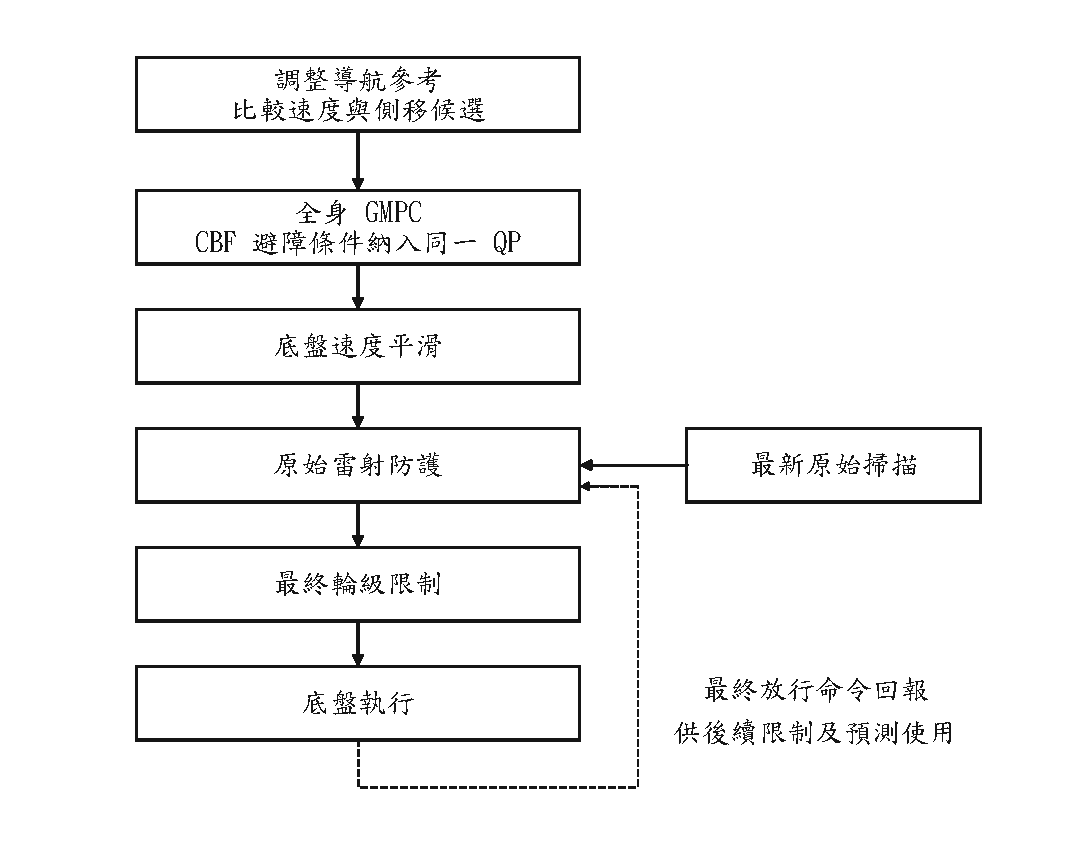
\includegraphics[width=0.98\textwidth]{figsrc/ch03/navigation_command_layers.pdf}
    \caption{導航參考調整、預測避障與底盤命令處理之分層關係}
    \label{fig:ch3_navigation_command_layers}
\end{figure}


% ==================================================
% 3.5.1 Mask R-CNN 原論文架構
% 位置：3.5.1 六類模型與訓練資料介紹之後、各物件深度估測之前
% 正文來源：03_05_visual_task_reference.tex
% 同名 PDF 請覆蓋上傳；同名 label 只保留一份。
% ==================================================
Mask R-CNN 的原始流程如\cref{fig:ref_mask_rcnn_framework}所示，對候選區域同時提供類別、外框與實例遮罩。此圖用於說明原方法概念；本研究採用前述 ResNet-50-FPN v2 實作，並將遮罩連結至深度幾何估測。
\begin{figure}[htbp]
    \centering
    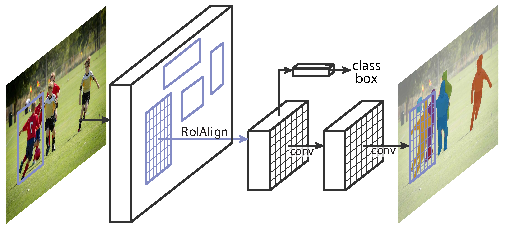
\includegraphics[width=0.95\textwidth]{figsrc/reference_figures/mask_rcnn_framework_he2017.pdf}
    \caption{Mask R-CNN 實例分割方法之原理示意（引自文獻\cite{he2017maskrcnn}之圖~1）}
    \label{fig:ref_mask_rcnn_framework}
\end{figure}


% ==================================================
% 3.5.1 本研究視覺目標生成流程
% 位置：3.5.1 深度反投影及各物件幾何估測說明之後、3.5.2 之前
% 正文來源：03_05_visual_task_reference.tex
% 同名 PDF 請覆蓋上傳；同名 label 只保留一份。
% ==================================================
本研究由分割至操作目標的資料流程如\cref{fig:ch3_mask_rcnn_target_pipeline}所示。遮罩與同一畫面的深度對應後，先建立相機座標中的幾何量，再以影像擷取時間對齊機器人狀態與相機外參，得到帶有來源時間的世界座標目標。門把分支保留擴張 ROI 所需的背景深度，各類目標依其幾何特性採用相應估測。
\begin{figure}[htbp]
    \centering
    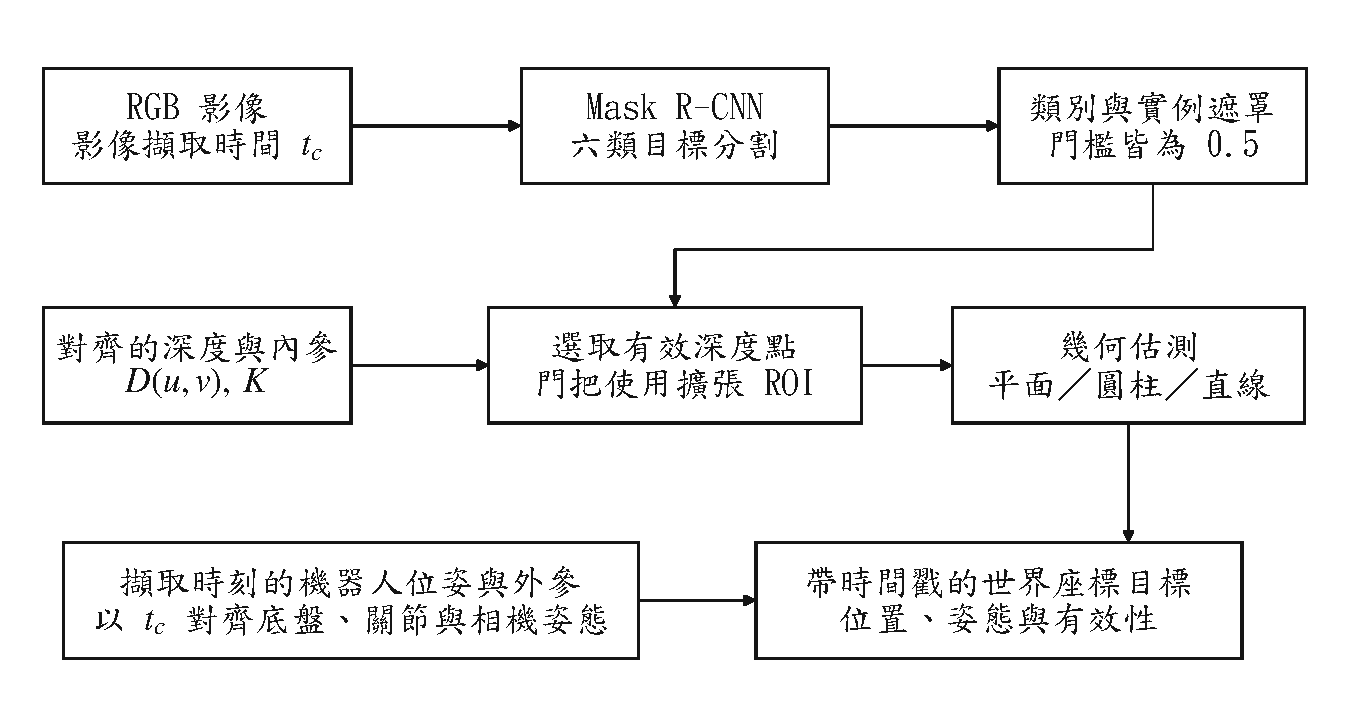
\includegraphics[width=0.98\textwidth]{figsrc/ch03/mask_rcnn_target_pipeline.pdf}
    \caption{本研究之實例分割、深度點選取與帶時間戳操作目標生成流程}
    \label{fig:ch3_mask_rcnn_target_pipeline}
\end{figure}


% ==================================================
% 3.5.2 影像與機器人狀態時間對齊
% 位置：3.5.2 帶時間戳的座標轉換與有效性說明之後
% 正文來源：03_05_visual_task_reference.tex
% 同名 PDF 請覆蓋上傳；同名 label 只保留一份。
% ==================================================
視覺量測與相機位姿的時間配對如\cref{fig:ch3_visual_time_alignment}所示。影像處理完成後仍保留原觀測時間 $t_o$，並使用該時刻的相機位姿進行座標轉換，再將世界座標中的目標提供給操作參考生成。
\begin{figure}[htbp]
    \centering
    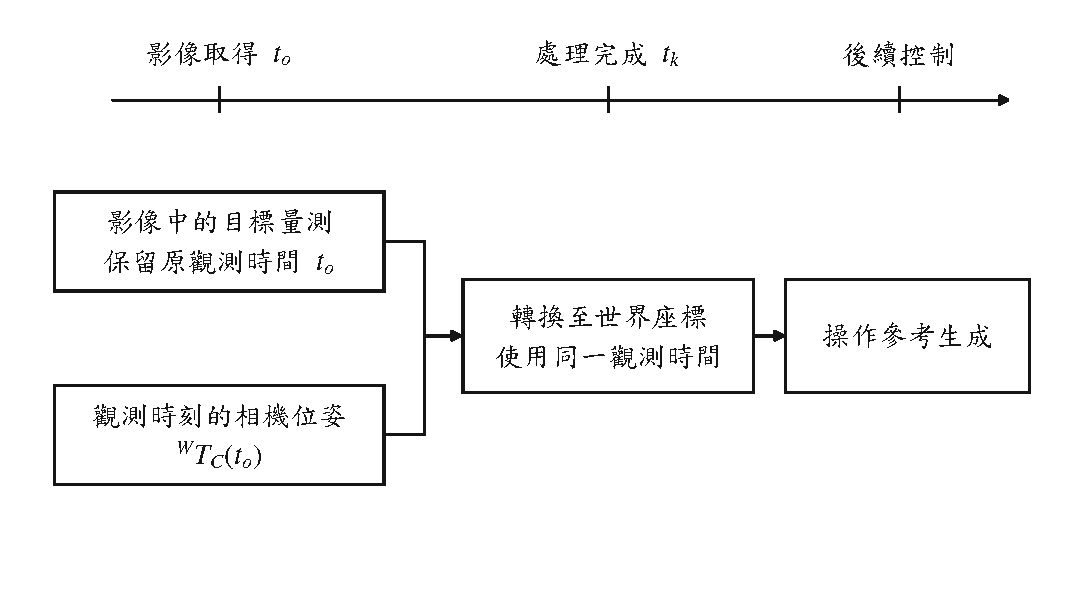
\includegraphics[width=0.98\textwidth]{figsrc/ch03/visual_time_alignment.pdf}
    \caption{視覺量測與相機位姿依觀測時間配對之流程}
    \label{fig:ch3_visual_time_alignment}
\end{figure}


% ==================================================
% 3.5.3 操作目標與底盤選位
% 位置：3.5.3 候選集合、評分式與選位機制之後
% 正文來源：03_05_visual_task_reference.tex
% 同名 PDF 請覆蓋上傳；同名 label 只保留一份。
% ==================================================
底盤選位前後的操作關係如\cref{fig:ch3_visual_operation_reference}所示。系統依已定位目標與家具幾何產生底盤候選，通過淨空、路線與手臂構型檢查後，再依評分選擇操作位姿。選定結果提供導航接近目標與可用手臂構型，後續仍依實際狀態更新控制參考。
\begin{figure}[htbp]
    \centering
    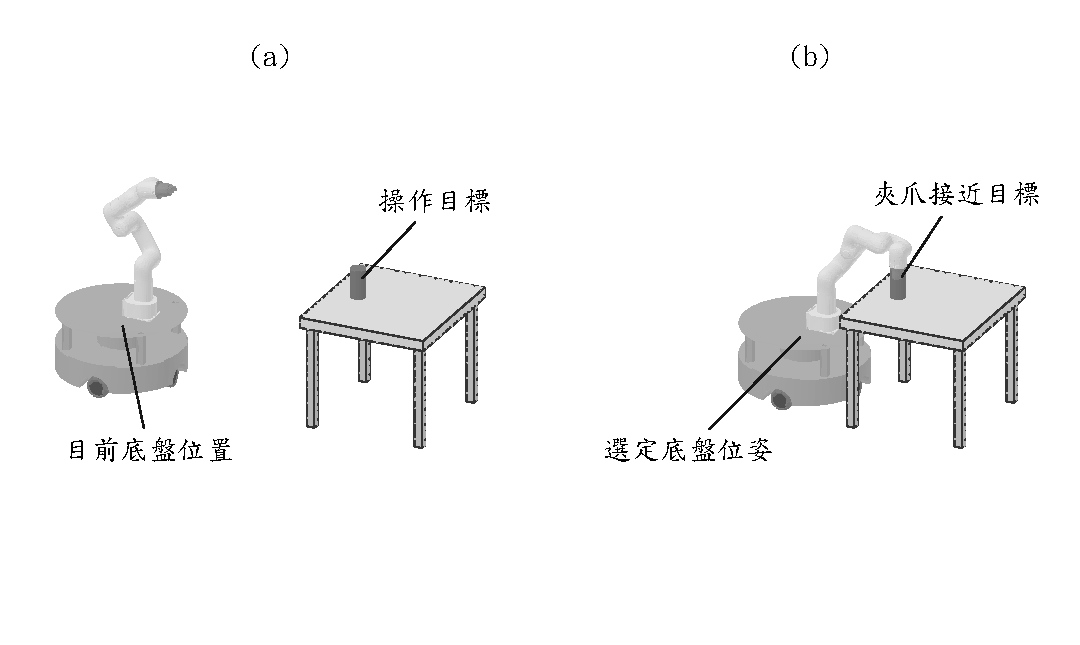
\includegraphics[width=0.98\textwidth]{figsrc/ch03/visual_operation_reference.pdf}
    \caption{操作目標導引之底盤選位：(a) 選位前的機器人與目標位置；(b) 選位後，手臂接近目標。}
    \label{fig:ch3_visual_operation_reference}
\end{figure}


% ==================================================
% 3.5.4 移動中接近的距離剖面
% 位置：3.5.4 關節展開、後段併線及距離限速說明之後；3.6.1 只引用此圖
% 正文來源：03_05_visual_task_reference.tex
% 同名 PDF 請覆蓋上傳；同名 label 只保留一份。
% ==================================================
\cref{fig:ch3_mobile_approach_distance_profile}以第 101 趟圓柱參考封包的參數說明距離剖面。逐軸平移速度上限在剩餘距離 $1.3$ 至 $0.4$ m 間，以三次平滑函數由 $0.26$ 降至 $0.06$ m/s；距離展開進度則在 $1.2$ 至 $0.3$ m 間由零增加至一，超過 $\beta_0=0.55$ 後逐步併入抓取線。圖中顯示距離規則的設計曲線，實際進度另受最短展開時間限制，最終速度由導航、障礙、家具鄰近條件及輪級限制共同決定。閉爪與確認仍依實測到位及抓持條件觸發。
\begin{figure}[htbp]
    \centering
    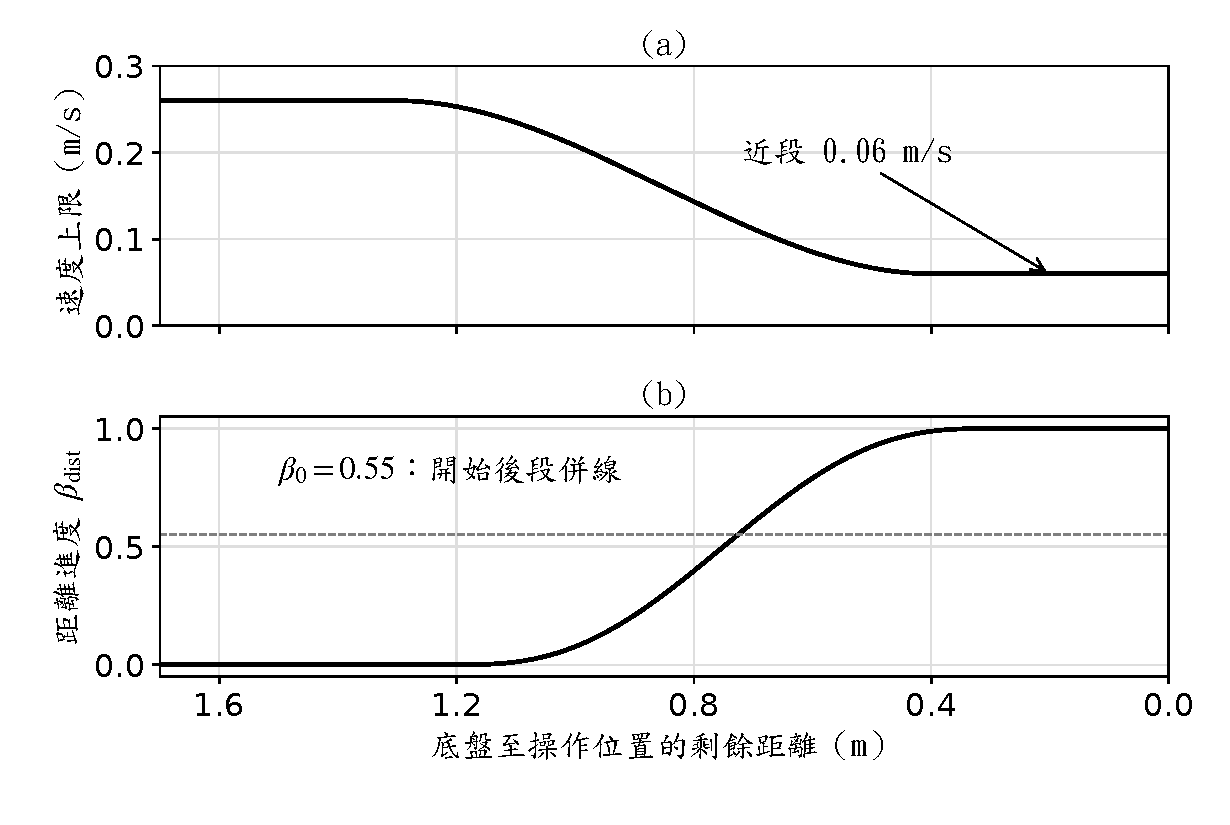
\includegraphics[width=0.94\textwidth]{figsrc/ch03/mobile_approach_distance_profile.pdf}
    \caption{圓柱接近階段之距離規則：(a) 平移逐軸速度上限；(b) 手臂距離展開進度與後段併線門檻。圖中為設計曲線，實際進度另受時間與狀態限制。}
    \label{fig:ch3_mobile_approach_distance_profile}
\end{figure}


% ==================================================
% 3.6.1 接近、閉爪與抓持確認
% 位置：3.6.1 抓持證據與理想連接確認說明之後
% 正文來源：03_06_mobile_constrained_operation.tex
% 同名 PDF 請覆蓋上傳；同名 label 只保留一份。
% ==================================================
抓持狀態的轉移如\cref{fig:ch3_grasp_state_transition}所示。閉爪命令發出後，需檢查手指位置與接觸證據，待條件持續成立並取得必要的連接確認後，才銜接抓持後的機構操作或持物運送。
\begin{figure}[htbp]
    \centering
    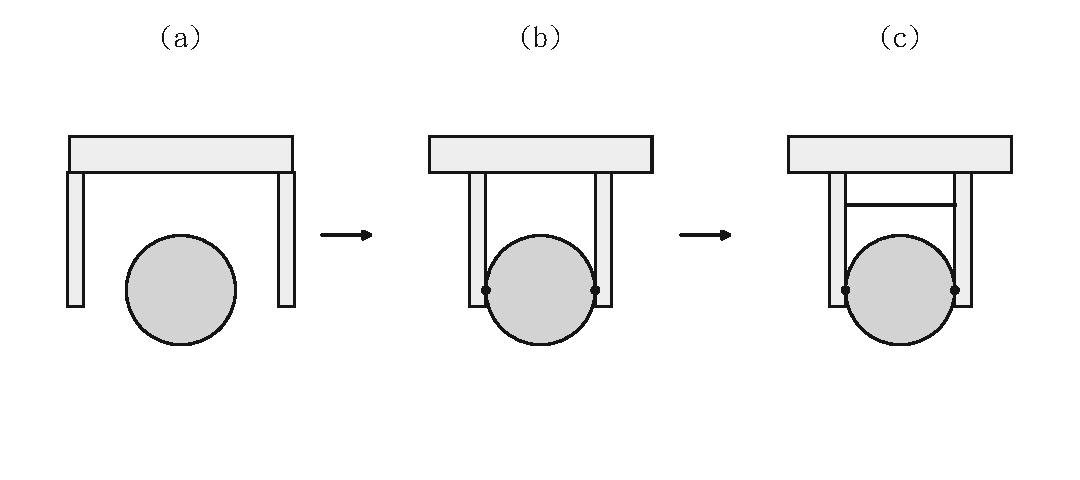
\includegraphics[width=0.98\textwidth]{figsrc/ch03/grasp_state_transition.pdf}
    \caption{抓持狀態之轉移：(a) 張爪接近目標；(b) 閉爪並檢查抓持證據；(c) 證據持續達標且取得必要的連接確認後，進入抓持狀態。}
    \label{fig:ch3_grasp_state_transition}
\end{figure}


% ==================================================
% 3.6.2 開門前後的全身構型
% 位置：3.6.2 旋轉門模型及門角更新公式之後
% 正文來源：03_06_mobile_constrained_operation.tex
% 同名 PDF 請覆蓋上傳；同名 label 只保留一份。
% ==================================================
不同門角下的協同構型如\cref{fig:ch3_door_operation_sequence}所示。把手繞鉸鏈運動時，底盤位置與手臂構型配合調整，並維持式\eqref{eq:ch3_grasp_closed_chain}所定義的抓持相對位姿。
\begin{figure}[htbp]
    \centering
    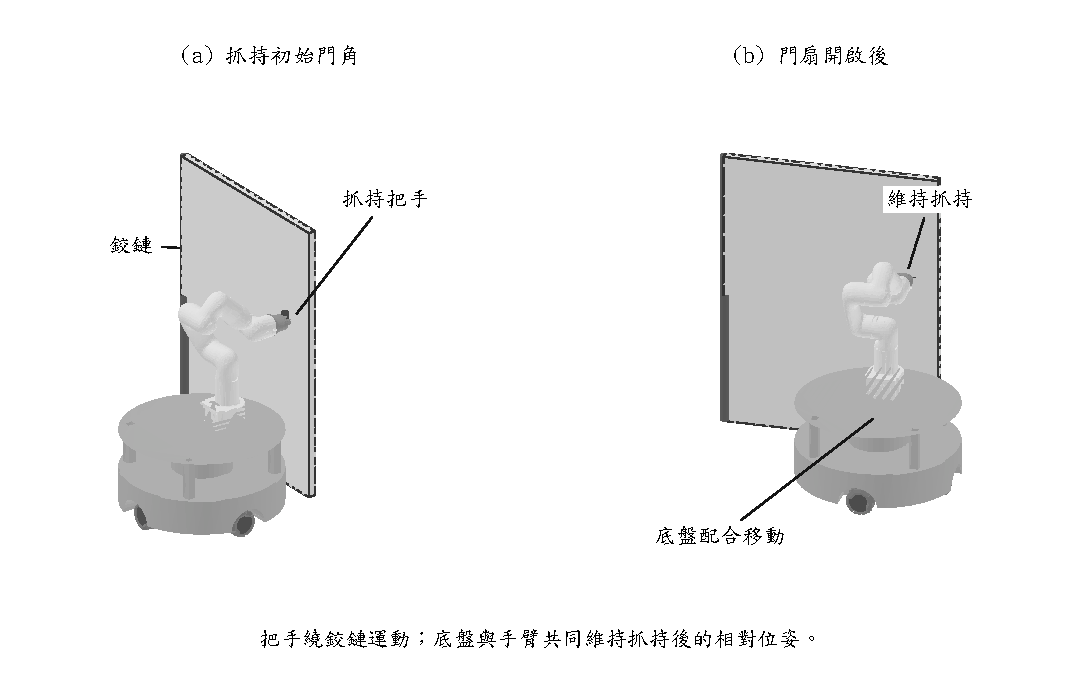
\includegraphics[width=0.98\textwidth]{figsrc/ch03/door_operation_sequence.pdf}
    \caption{門扇操作之全身構型：(a) 抓持初始門角；(b) 門扇開啟後，底盤與手臂配合把手運動。}
    \label{fig:ch3_door_operation_sequence}
\end{figure}


% ==================================================
% 3.6.2 抽屜拉出前後的全身構型
% 位置：3.6.2 平移抽屜模型及行程限制公式之後
% 正文來源：03_06_mobile_constrained_operation.tex
% 同名 PDF 請覆蓋上傳；同名 label 只保留一份。
% ==================================================
抽屜拉出前後的機構位移與全身構型如\cref{fig:ch3_drawer_operation_sequence}所示。抽屜沿滑軌平移並保持機構姿態，底盤與手臂則依操作進度更新參考，以維持抓持及所需的運動空間。
\begin{figure}[htbp]
    \centering
    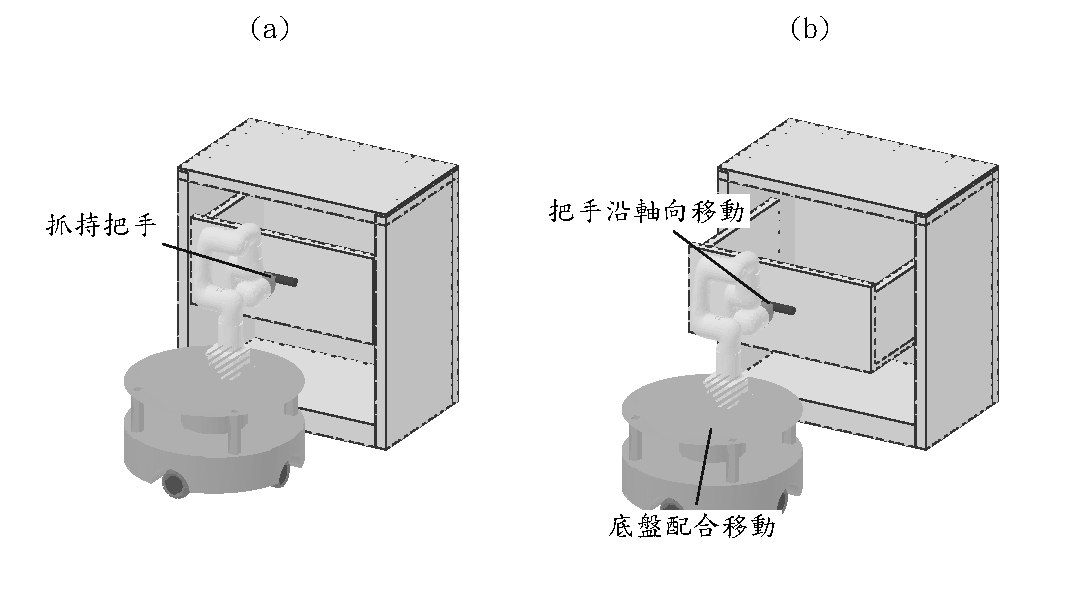
\includegraphics[width=0.98\textwidth]{figsrc/ch03/drawer_operation_sequence.pdf}
    \caption{抽屜操作之全身構型：(a) 抽屜初始位置；(b) 抽屜沿滑軌拉出後，底盤與手臂配合調整。}
    \label{fig:ch3_drawer_operation_sequence}
\end{figure}


% ==================================================
% 3.6.3 相對底盤的持物運送
% 位置：3.6.3 底盤相對持物目標公式與流程說明之後
% 正文來源：03_06_mobile_constrained_operation.tex
% 同名 PDF 請覆蓋上傳；同名 label 只保留一份。
% ==================================================
相對底盤目標下的運送關係如\cref{fig:ch3_base_relative_carrying}所示。手臂維持相對底盤的末端構型時，物件在世界座標中的位置隨底盤一起改變。此關係由式\eqref{eq:ch3_base_relative_carry_target}建立，與前述世界固定操作目標分別處理。
\begin{figure}[htbp]
    \centering
    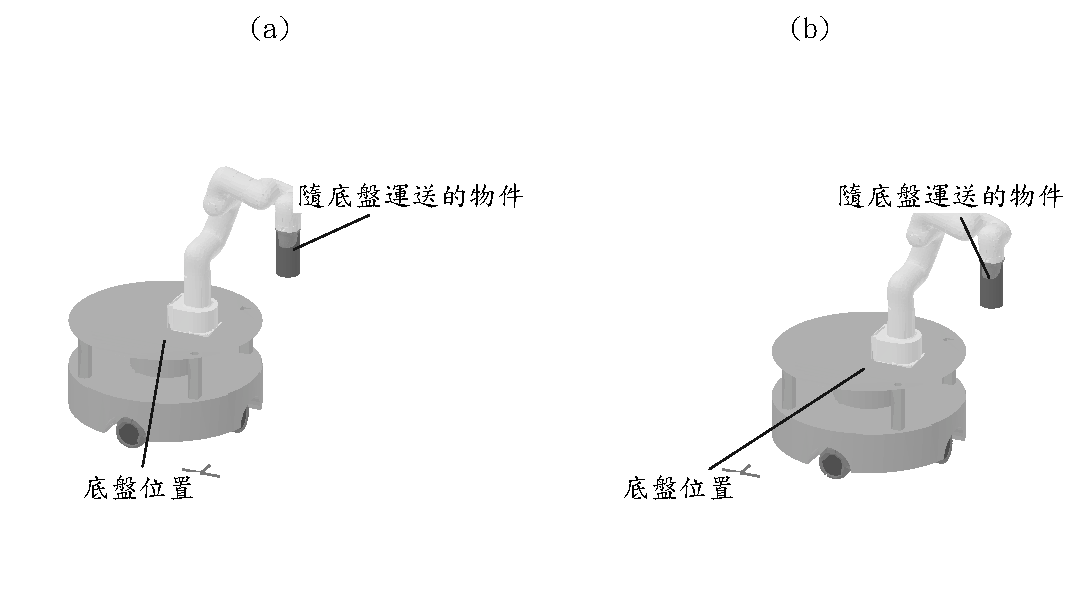
\includegraphics[width=0.98\textwidth]{figsrc/ch03/base_relative_carrying.pdf}
    \caption{相對底盤目標下之持物運送：(a) 底盤移動前；(b) 底盤平移後，維持相同的底盤相對末端構型。}
    \label{fig:ch3_base_relative_carrying}
\end{figure}


% ==================================================
% 3.7.1 命令在途、接續與停止時序
% 位置：3.7.1 在途命令前推及生效初始狀態說明之後
% 正文來源：03_07_execution_compensation.tex
% 同名 PDF 請覆蓋上傳；同名 label 只保留一份。
% ==================================================
控制計算與命令接續的時序如\cref{fig:ch3_command_execution_timeline}所示。計算期間既定命令持續執行，控制器依其作用預測新控制段生效時刻的狀態。新結果通過期限與可行性核對後才接續執行；若拒絕或逾時，則沿已核對的停止尾段減速。
\begin{figure}[htbp]
    \centering
    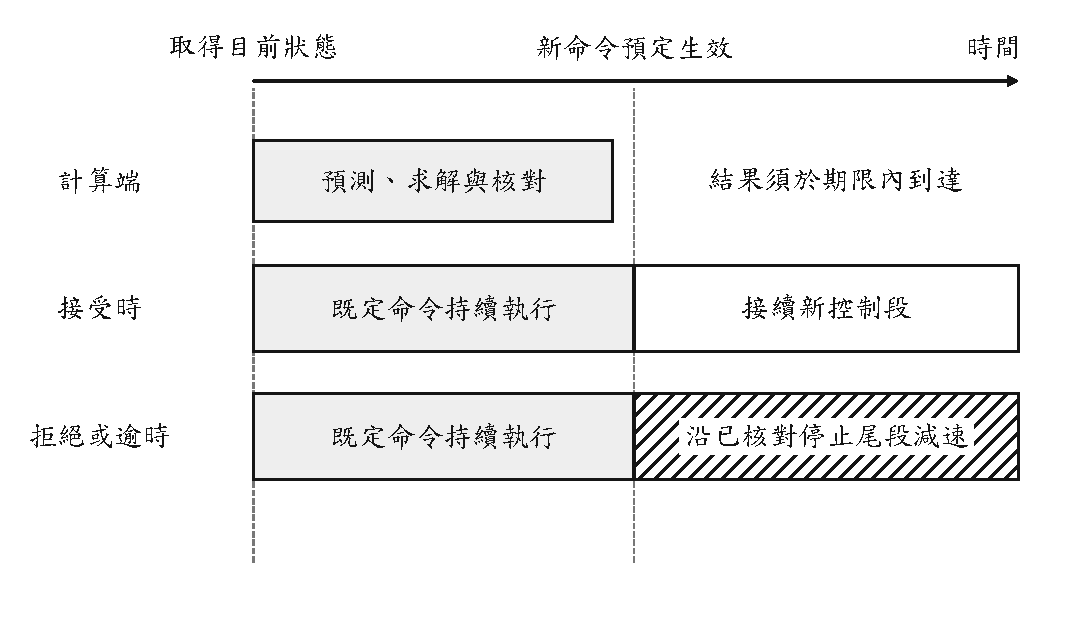
\includegraphics[width=0.98\textwidth]{figsrc/ch03/command_execution_timeline.pdf}
    \caption{控制計算期間之命令接續與停止備援}
    \label{fig:ch3_command_execution_timeline}
\end{figure}


% ==================================================
% 3.7.2 模型偏置估測
% 位置：3.7.2 偏置觀測、平滑及限幅公式之後，TCP 補償介紹之前
% 正文來源：03_07_execution_compensation.tex
% 同名 PDF 請覆蓋上傳；同名 label 只保留一份。
% ==================================================
模型偏置估測的更新位置如\cref{fig:ch3_model_bias_estimation}所示。區間末殘差先由更新前的偏置估計計算，經平滑與限幅後，再將新偏置提供給後續 QP 預測、在途命令前推與停止軌跡核對使用。
\begin{figure}[htbp]
    \centering
    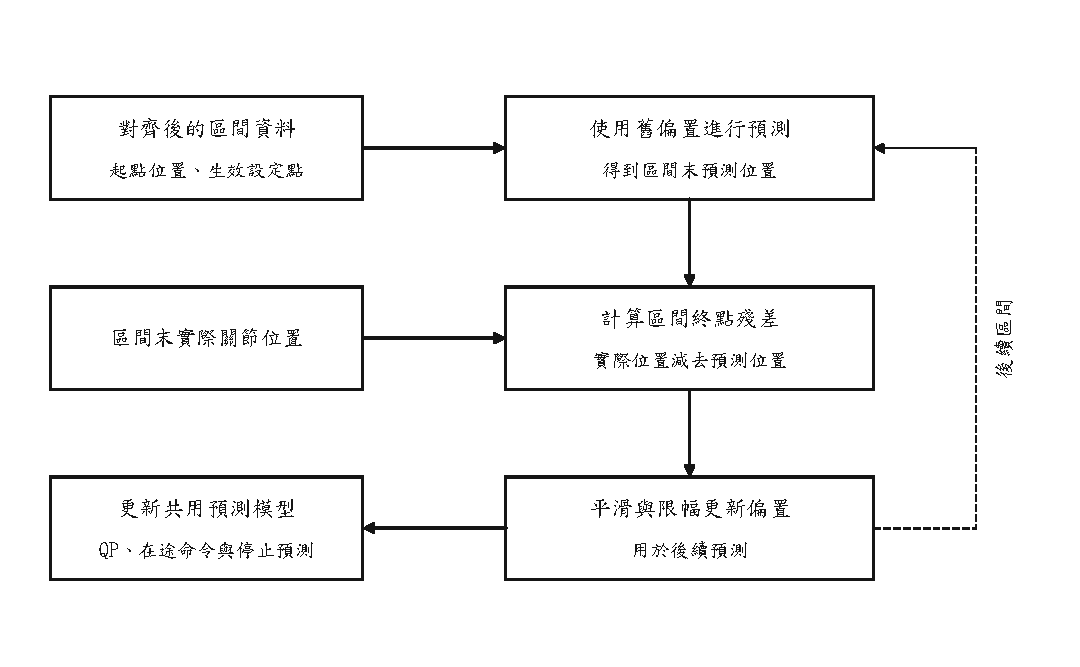
\includegraphics[width=0.98\textwidth]{figsrc/ch03/model_bias_estimation.pdf}
    \caption{模型偏置估測之區間殘差與共用模型更新}
    \label{fig:ch3_model_bias_estimation}
\end{figure}


% ==================================================
% 3.7.2 TCP 有界目標補償
% 位置：3.7.2 TCP 積分補償公式及完成條件說明之後
% 正文來源：03_07_execution_compensation.tex
% 同名 PDF 請覆蓋上傳；同名 label 只保留一份。
% ==================================================
末端目標修正的作用如\cref{fig:ch3_tcp_target_compensation}所示。圖中以單一位置分量說明原始幾何目標、實際末端位置及補償後命令目標的差異；補償量只改變控制器追蹤的命令目標，完成條件仍以原始幾何目標判定。
\begin{figure}[htbp]
    \centering
    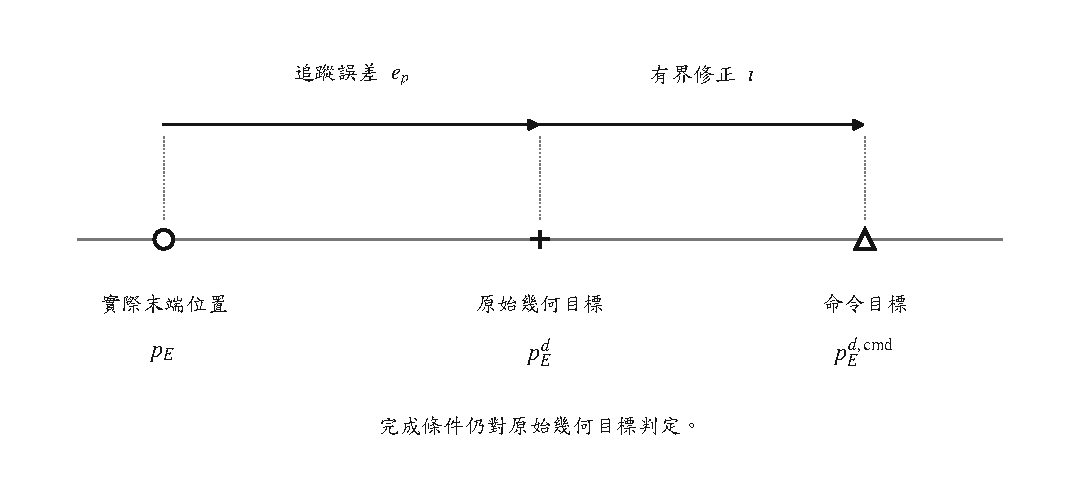
\includegraphics[width=0.98\textwidth]{figsrc/ch03/tcp_target_compensation.pdf}
    \caption{末端原始幾何目標與有界命令目標補償；完成條件依原始幾何目標判定。}
    \label{fig:ch3_tcp_target_compensation}
\end{figure}


% ==================================================
% 3.7.4 全身預測控制完整流程
% 位置：3.7.4 第一段之後、演算法框之前
% 正文來源：03_07_execution_compensation.tex
% 同名 PDF 請覆蓋上傳；同名 label 只保留一份。
% ==================================================
整體控制流程如\cref{fig:ch3_wholebody_control_workflow}所示。系統由狀態與感知更新開始，建立生效起點與任務參考後求解全身 GMPC，再依候選核對結果執行新控制段或停止備援，最後以實際命令與新狀態形成回授。
\begin{figure}[htbp]
    \centering
    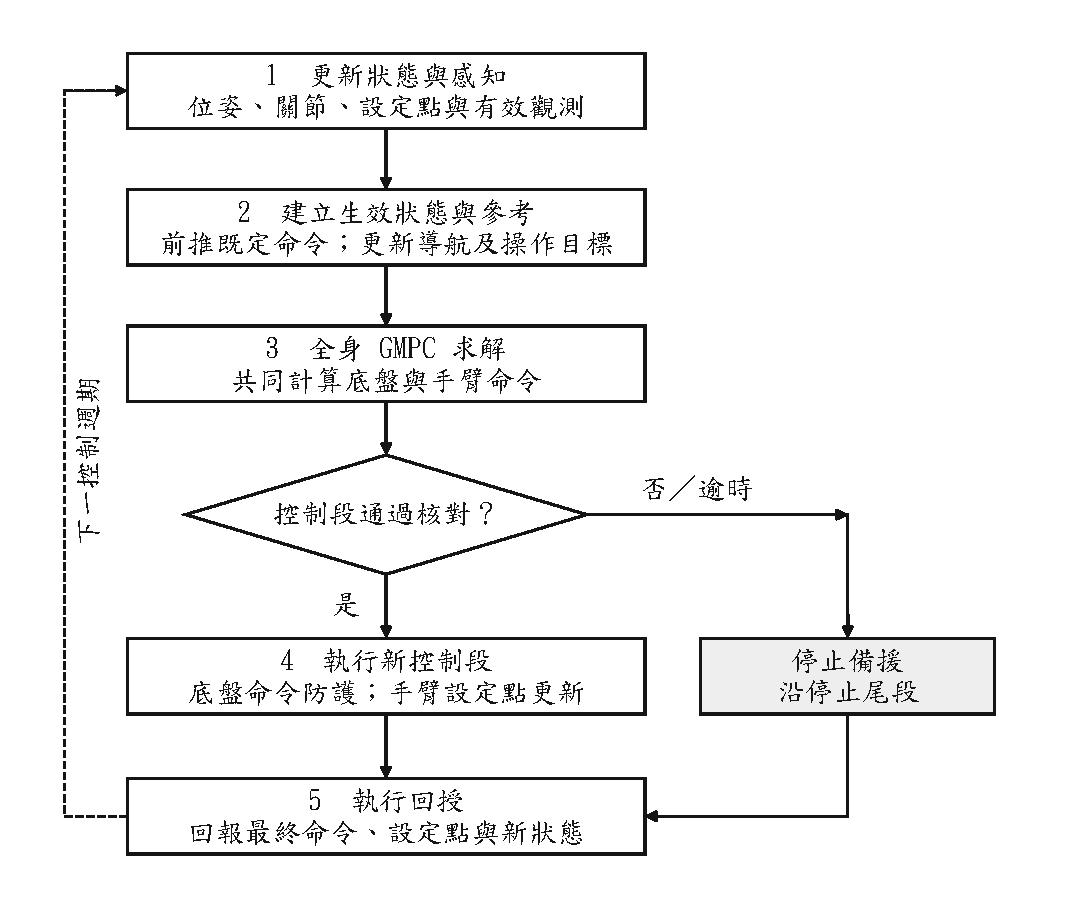
\includegraphics[width=0.98\textwidth]{figsrc/ch03/wholebody_control_workflow.pdf}
    \caption{全身預測控制之計算、命令核對與執行回授流程}
    \label{fig:ch3_wholebody_control_workflow}
\end{figure}

